RNA modifications have emerged as pivotal regulators of gene expression and cellular function.
Among these modifications, pseudouridine (\pseudo) stands out as the most abundant and one of the earliest discovered nucleoside modifications in RNA~\cite{charette_pseudouridine_2000}.
This research focuses on developing computational models using machine learning (ML) and deep learning (DL) algorithms to predict pseudouridine sites within RNA sequences.
By accurately identifying these sites, we aim to enhance the understanding of pseudouridylation's role in biology and its implications in human diseases, thereby facilitating the development of novel diagnostic and therapeutic strategies.


\section{Overview}\label{sec:overview}
  Pseudouridine (\pseudo), a modified nucleoside, is the 5-ribosyl isomer of uridine and is the most common RNA modification across various RNA types.
  It was first discovered in transfer RNA (tRNA), but its presence has been identified in ribosomal RNA (rRNA), small nuclear RNA (snRNA), and messenger RNA (mRNA)~\cite{cohn_nucleoside-5-phosphates_1951}.

  Pseudouridine formation occurs through a process called pseudouridylation, catalyzed by enzymes known as pseudouridine synthases.
  During this modification, the nitrogen-carbon (N\textminus{C}) glycosidic bond of uridine is rearranged into a carbon-carbon (C\textminus{C}) glycosidic bond.
  This modification changes the structural properties of RNA, allowing pseudouridine to participate in enhanced hydrogen bonding and increase RNA stability~\cite{charette_pseudouridine_2000}.

  The key structural difference between uridine and pseudouridine lies in this glycosidic bond.
  While uridine has a nitrogen atom at position 1 connected to the ribose sugar, pseudouridine has a carbon atom at position 5 linked to the ribose, which provides additional hydrogen bonding capabilities.
  This structural change reinforces the RNA backbone and contributes to the overall stabilization of RNA molecules, making pseudouridine important in maintaining RNA function and conformation~\cite{ge_rna_2013}.

  \begin{figure}[h!]
    \centering
    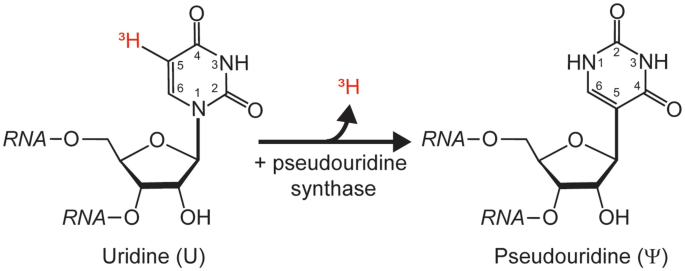
\includegraphics[width=.7\textwidth]{images/psi-synthesis}
%    \chemname{
%      \chemfig[cram width=2pt]{HO?<[:-60](-[6]OH)-[,,,,line width=2pt](-[6]OH)>[:60]-[:150, 1.1]O?}
%    }{Uridine}
%
%    \chemname{
%      \chemfig{*6((=O)-N-(*5(-N=-N(-H)-))=-(=O)-N(-H)-)}
%    }{Pseudouridine}

    \caption{Chemical structure of uridine and pseudouridine with numbering of selected atoms.}
    \label{fig:structure-pseudouridine}
  \end{figure}

  \textbf{Figure~\ref{fig:structure-pseudouridine}} provides a comparison of the structures of uridine and pseudouridine, highlighting the key difference in glycosidic bond placement.
